\chapter{Validation}
\label{validation}

This chapter is split into two parts. First we are going to state how we are going to validate in the methodology section, before performing the actual validation of our requirements on our solution.


\section{Methodology}
\label{validation_methodology}
In this section we will build our validation methodology by choosing an accurate test environment, and defining our scenarios, measurements and experiments.

\subsection{Test environment}
As a test environment we want to use a network emulator to be able to easily bootstrap our solution. For this, multiple emulators are available, including mininet \cite{mininet}, distrinet \cite{distrinet1, distrinet2}, maxinet \cite{maxinet}, ComNetsEmu \cite{comnetsemu} or our own testbed solution \cite{owntb}.

\paragraph{Mininet and ComNetsEmu} emulate network topologies on a single machine, but do not scale to multiple machines. As we want to test in a distributed setting, they are unfortunately out of the equation.

\paragraph{Distrinet and maxinet} would both allow us to scale mininet topologies to multiple machines. As we want to be able to deploy our topologies to real-world devices in the future though and integrate real-world hardware (requirement R3), we would need to invest additional effort in deploying to real-world hardware in the future when using them.

\paragraph{Our own testbed solution} mitigates these issues by supporting multiple modes of deployment including support for real-world hardware that can easily be extended.

\paragraph{} We will thus opt to use our own hybrid testbed to evaluate our solution.

\subsection{Scenarios}
\label{scenarios}
We will test three scenarios in total. The first scenario will provide a base case for our two other slicing-enabled scenarios, of which one will be local and the other distributed.

\begin{description}[style=multiline, labelwidth=0.7cm]
    \item[\namedlabel{S1}{S1}] \textbf{Reference scenario} The base solution will consist of two simulated hosts, two attackers and two switches. Each switch is connected to one of the hosts, one of the attackers and to the other switch. This scenario can be seen in Figure \ref{fig:scenario_1}.
    \begin{figure}[ht]
        \centering
        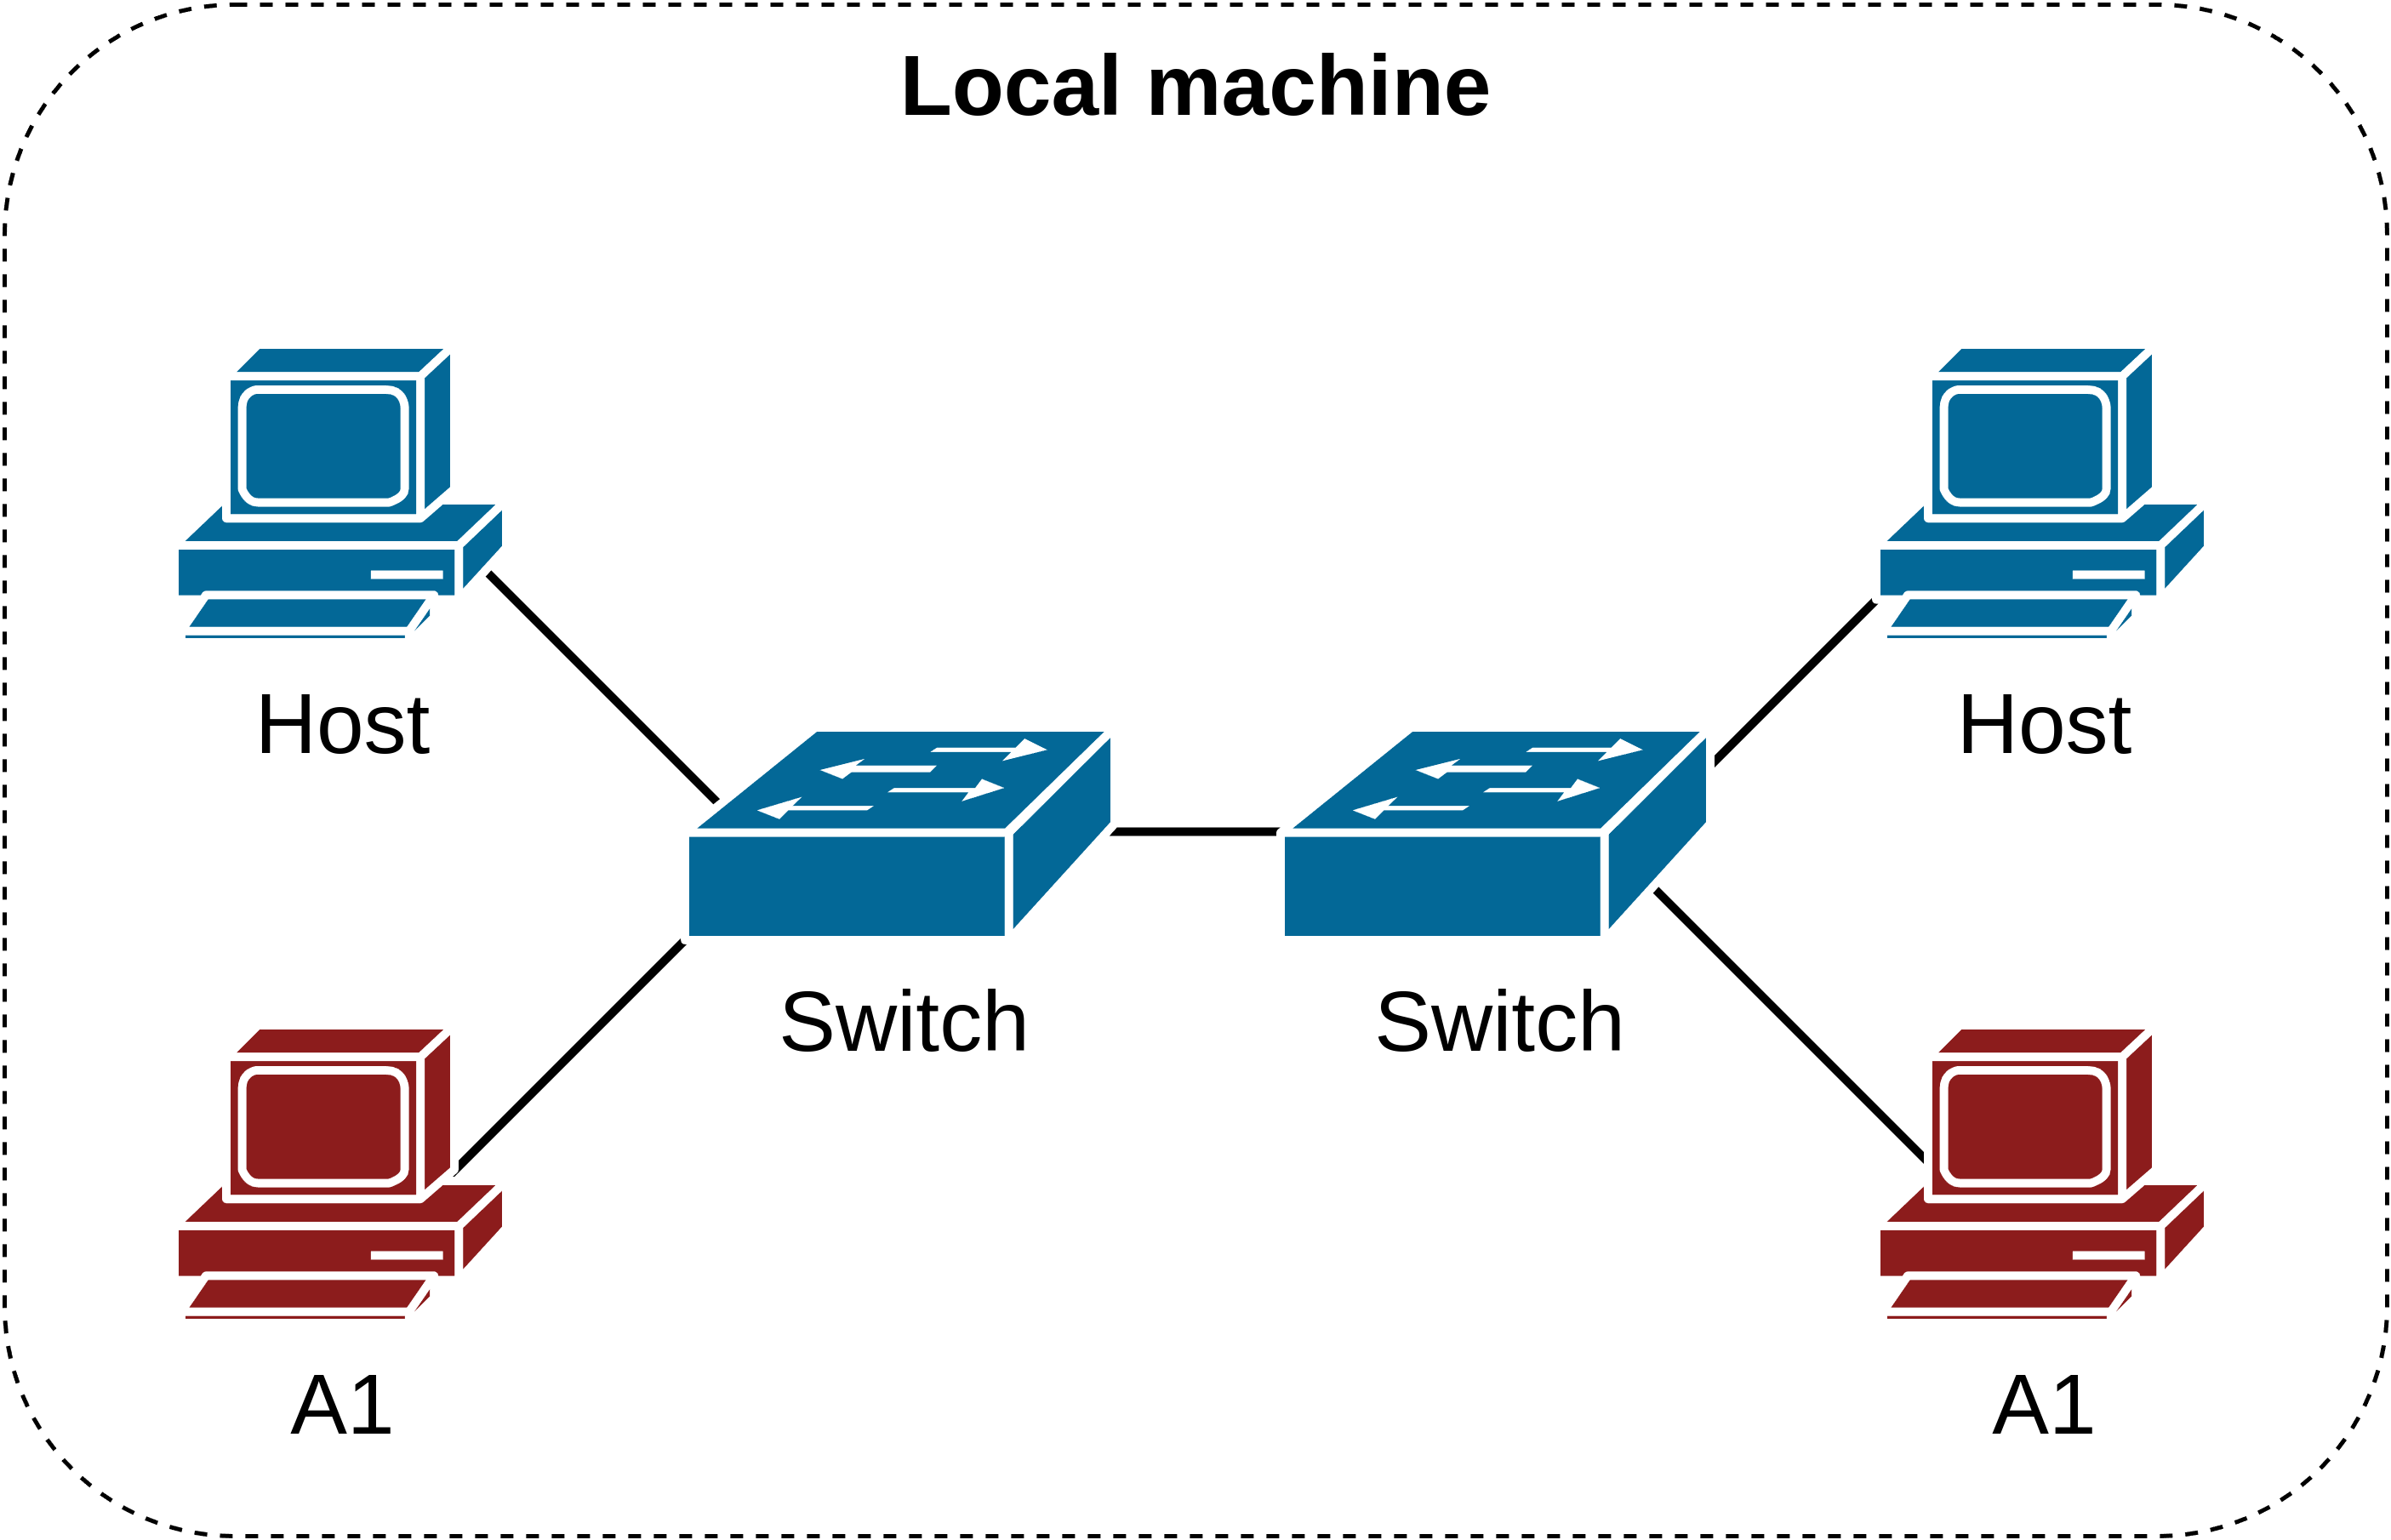
\includegraphics[width=6cm]{images/chapter_7/scenario_1.png}
        \caption[Validation Scenario 1]{Our first scenario \ref{S1} without network slicing.}
        \label{fig:scenario_1}
    \end{figure}
    \item[\namedlabel{S2}{S2}] \textbf{Local slicing scenario} For our first slicing scenario we will deploy our slicing solution emulating three domains with two \gls{edgenetwork}s and one black (semi-trusted) network between them. Each domain will have two slicing switches which the traffic of the slices has to pass. One of the simulated hosts will be created on each edge. This scenario can be seen in Figure \ref{fig:scenario_2}.
    \begin{figure}[ht]
        \centering
        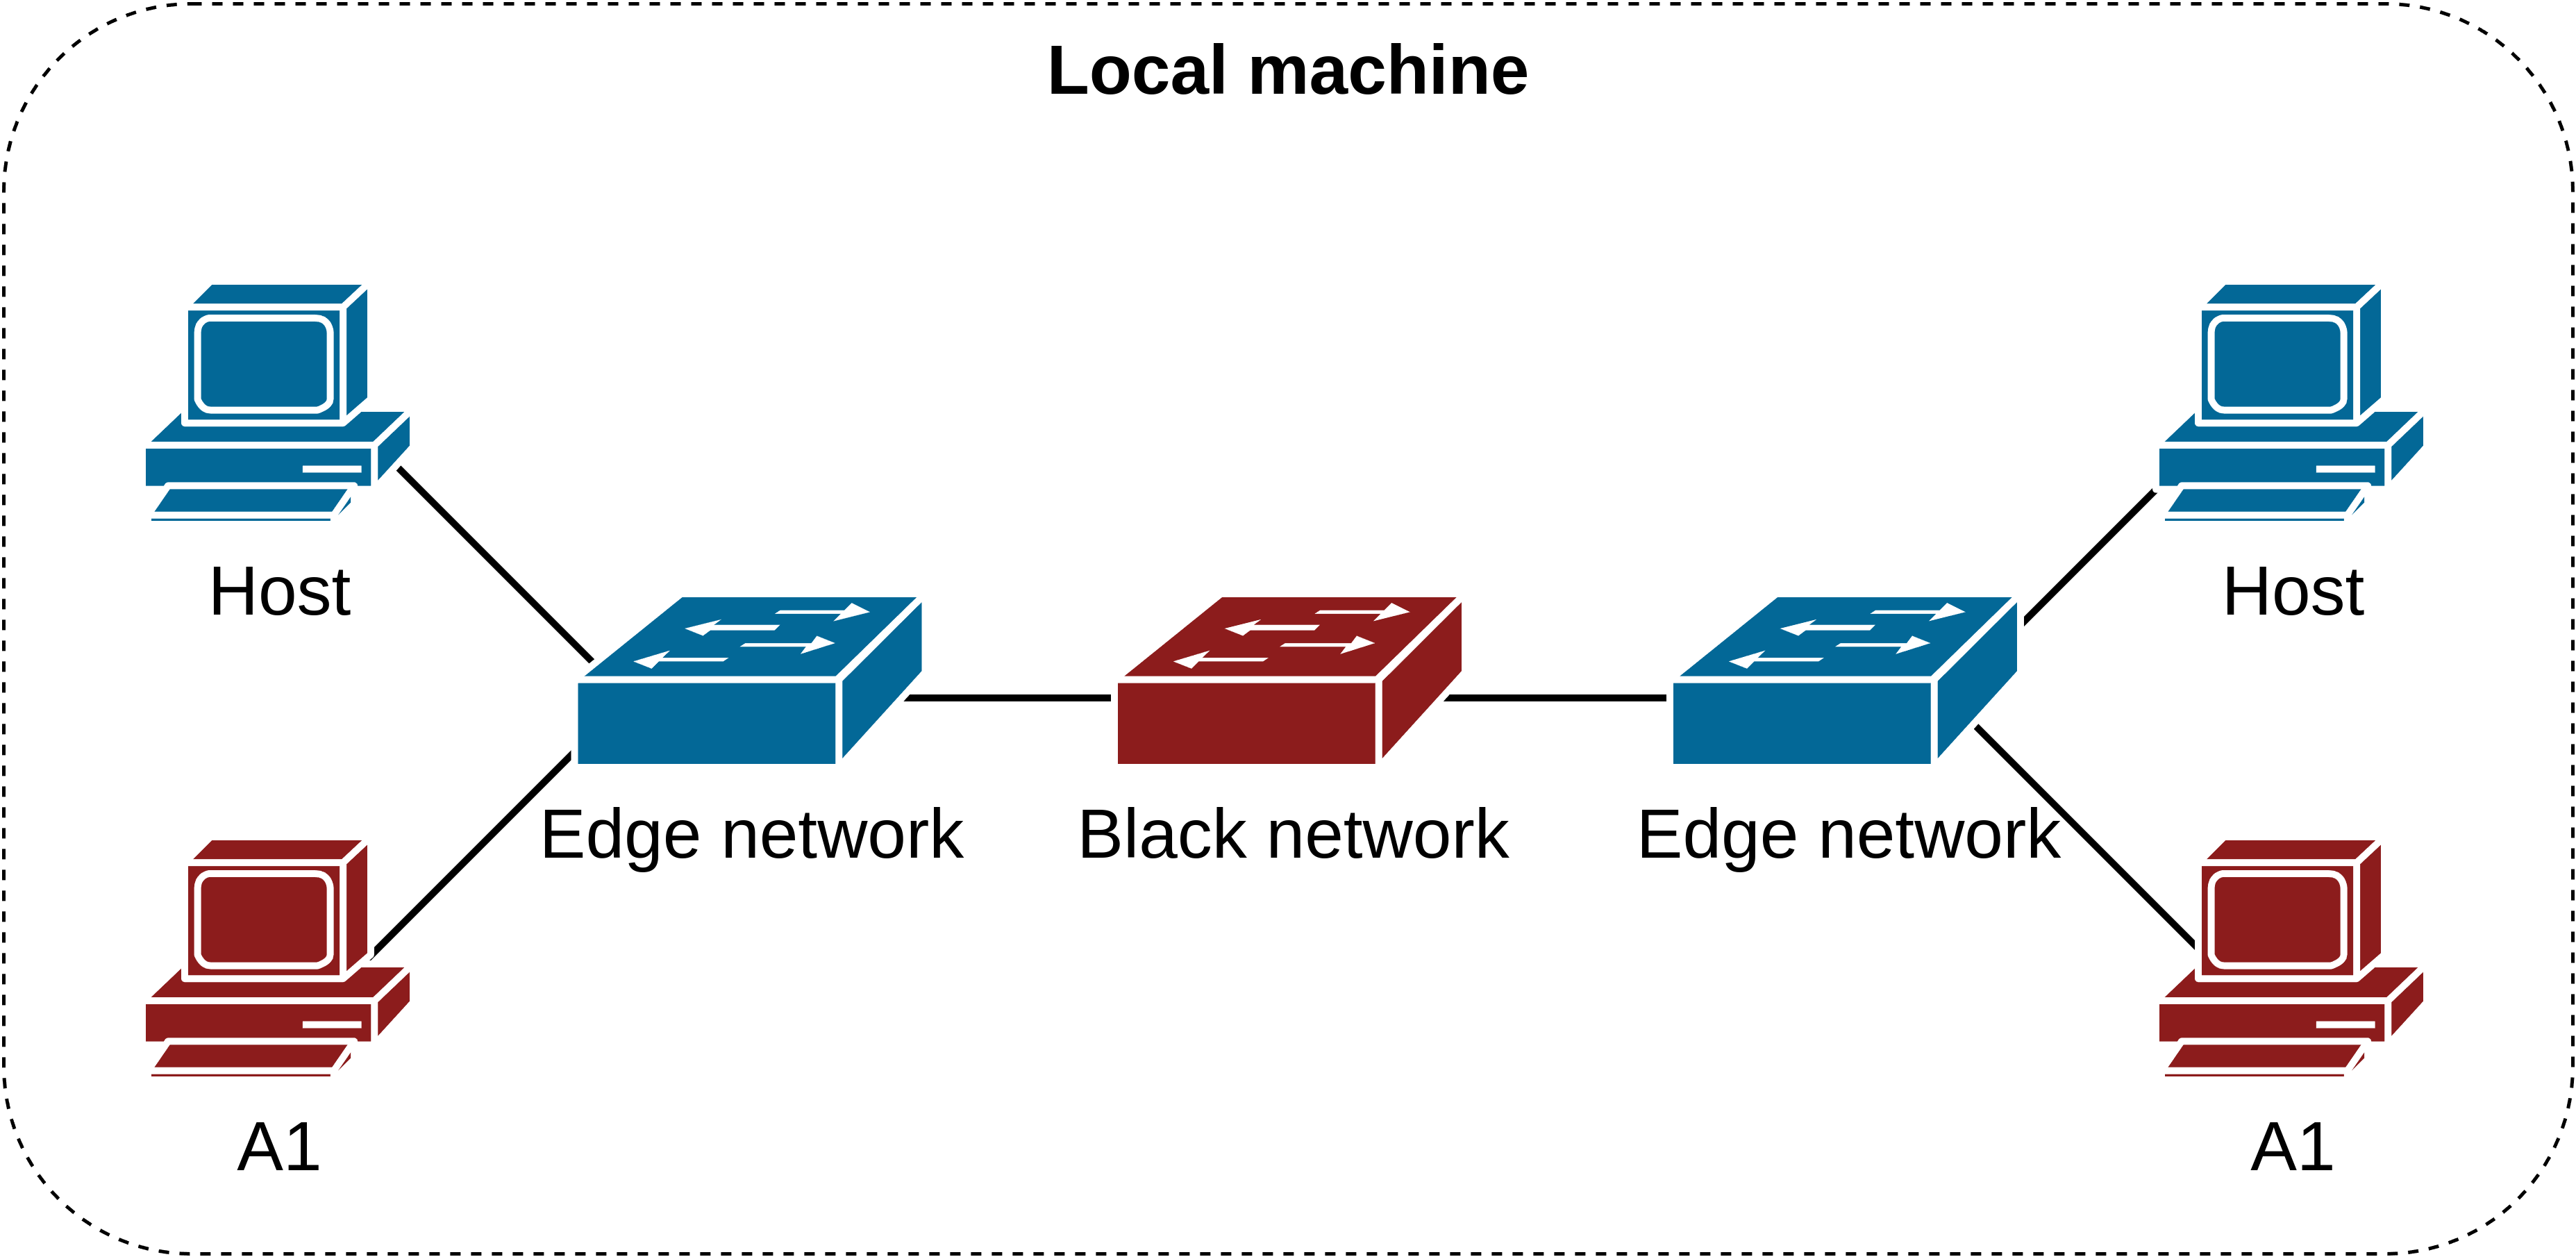
\includegraphics[width=8cm]{images/chapter_7/scenario_2.png}
        \caption[Validation Scenario 2]{Our second scenario \ref{S2} with network slicing across three domains running on a local test setup (one machine).}
        \label{fig:scenario_2}
    \end{figure}
    \item[\namedlabel{S3}{S3}] \textbf{Remote slicing scenario} As the last scenario we will deploy the previous scenario to three different servers that are connected via 10G links to an Aruba 2930F switch. Each server will contain one entire simulated domain. We hope that by this scenario we can observe some real-world performance characteristics when utilizing real links in our test environment. This scenario can be seen in Figure \ref{fig:scenario_3}.
    \begin{figure}[ht]
        \centering
        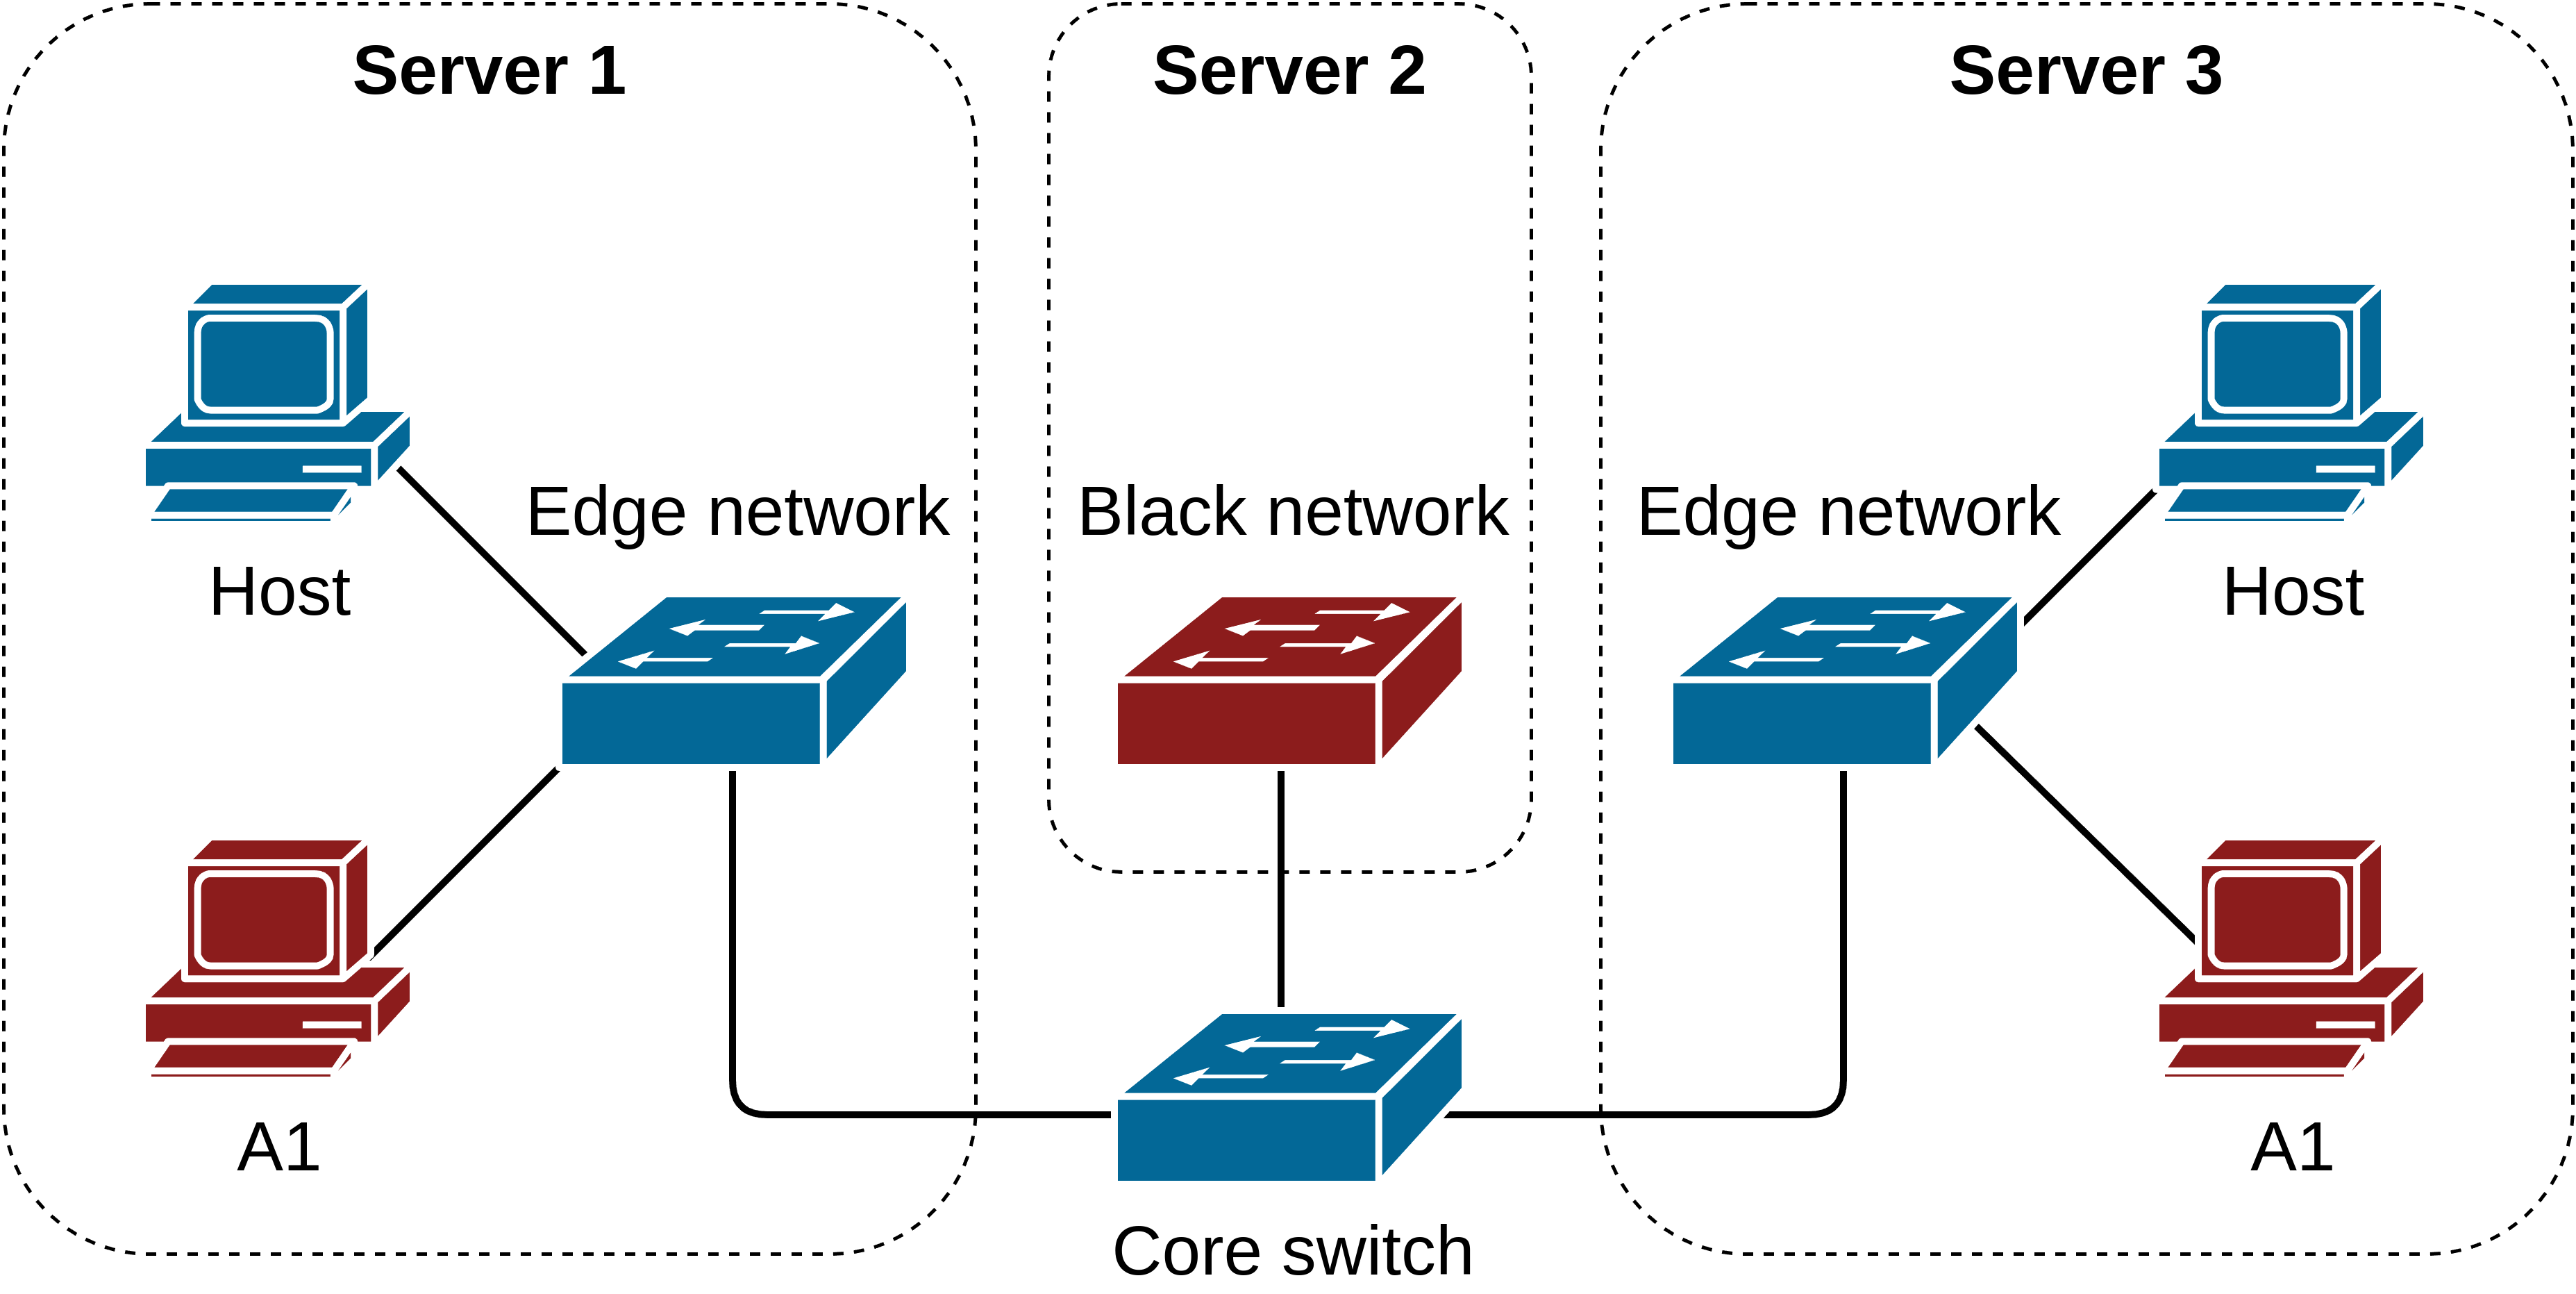
\includegraphics[width=8cm]{images/chapter_7/scenario_3.png}
        \caption[Validation Scenario 3]{Our last scenario \ref{S3} with network slicing across three domains, deploying one domain per server each. The three servers are connected via a switch.}
        \label{fig:scenario_3}
    \end{figure}
\end{description}

In each of our scenarios, all links will be limited to 1Gbit/s throughput by utilizing a token-bucket filter. In the local scenario \ref{S1}, the links attached to the attackers were limited to 2Gbit/s. The latter restriction was lifted in the other two scenarios to be able to attack with more traffic.

%The base solution will consist of two simulated hosts, two attackers and two switches. Each switch is connected to one of the hosts, one of the attackers and to the other switch. The attackers share the link between the switches with the normal host. The attacker \ref{A1} will then become active and attempt to disrupt the communication between the hosts. Furthermore we will employ attacker \ref{A4} to eavesdrop traffic between the switches. \ref{A2} and \ref{A3} do not apply since there is no slicing infrastructure.

%For our first slicing scenario we will deploy our slicing solution emulating 3 domains with two \gls{edgenetwork}s and one black (semi-trusted) network between them. We will place one attacker each in the edges to spam a slice between them as attacker \ref{A1}. We will deploy \ref{A4} on a link in the \gls{blacknetwork} and deploy \ref{A2} and \ref{A3} to the application plane.

%As the last scenario we will deploy the previous scenario to three different servers that are connected via 10G links to an Aruba 2930F switch. Each server will contain one entire simulated domain. We hope that by this scenario we can observe some real-world performance characteristics when utilizing real links in our test environment.

For each scenario we will try to establish two network slices in total. As an example, we want to control a robot on the other side by receiving a video stream and maintaining a bidirectional control and feedback stream, as in our use case for the surgery.

One slice will thus be unidirectional and streaming media content. We will allocate 8Mbit/s to this slice, because this encompasses streaming of HD video (according to the FCC \cite{fcc}). We require a relatively small \gls{lossrate} for this to not skip frames on the video stream, but loosing single packets and skipping a frame will not provide an essential problem. \Gls{jitter} may occur as we can buffer our video stream data for short amounts of time, however we want our \gls{latency} to be low so our frames appear in almost real time.

For the bidirectional control and feedback slice, we need far less \gls{bandwidth}. The \gls{lossrate} needs to be lower than with the video stream to be in control at all times. Also we require a low \gls{latency} and low \gls{jitter} to be able to react in real time and without any inaccurate movements. We will thus apply the resource guarantees in Table \ref{table:slices} to all of our scenarios.

\begin{table}[ht]
    \centering
    \begin{tabular}{ |c|c|c| }
        \hline
        \textbf{Metric} & \textbf{Media} & \textbf{Control} \\
        \hline
        \Gls{bandwidth} & $\geq$ 8Mbit/s & $\geq$ 100Kbit/s \\
        \Gls{latency}   & $<$ 5ms        & $<$ 3ms          \\
        \Gls{jitter}    & $<$ 0.5ms      & $<$ 0.3ms        \\
        \Gls{lossrate}  & $<$ 0.01\%     & $<$ 0.001\%      \\
        \hline
    \end{tabular}
    \caption[Slice \acrshort{qos} guarantees in our remote surgery example]{The guarantees we wish to meet with our slices concerning our remote surgery example.}
    \label{table:slices}
\end{table}

The robot example including the \gls{bandwidth} requirements is taken from Fuhrberg et al. \cite{SE4} in order to be able to compare their solution against our redesigned solution. The values for \gls{latency}, \gls{jitter} and \gls{lossrate} have been altered to reflect our goals and generally provide more strict requirements.

\subsection{Measurements}
\label{measurements}
Measurements on the resources of a slice will be performed by sending continuous traffic according to the slice specifications through the slice. By sending the traffic and observing the packets reaching the other end, we can obtain measurements on whether the slices upheld their guarantees in this specific situation or not.

To send the traffic and observe their result, we will use three different tools:

\paragraph{Iperf3} \cite{iperf3} is a network \gls{bandwidth} testing tool that also provides data on packet drops and connection \gls{jitter}. It supports both \acrshort{udp} and \acrshort{tcp}.

\paragraph{Iputils-ping} \cite{iputils} is a network \gls{latency} testing tool that provides data on \gls{latency}, packet drops and \gls{jitter}. We will not generate traffic using ping, but will rather use it for \gls{latency} measurements while \textit{iperf3} sends continuous traffic. It will use \acrshort{icmp} as protocol.

\paragraph{Sockperf} \cite{sockperf} is a network \gls{bandwidth} and \gls{latency} testing tool that provides data on \gls{bandwidth}, packet drops, \gls{latency} and \gls{jitter}. It supports both \acrshort{udp} and \acrshort{tcp}.

\paragraph{} More details on this can be seen in Table \ref{table:measurements}. We will thus be able to obtain each metric from at least two tools, providing us with the ability to verify their result.

\begin{table}[ht]
    \centering
    \begin{tabular}{ |c|c|c|c|c| }
        \hline
        \textbf{Tool} & \textbf{\Gls{bandwidth}} & \textbf{Packet drops} & \textbf{\Gls{latency}} & \textbf{\Gls{jitter}}  \\
        \hline
        IPerf3        & \ding{51}                & \acrshort{udp} only   & \acrshort{tcp} only    & \acrshort{udp} only   \\
        Ping          & \ding{55}                & \ding{51}             & \ding{51}              & \ding{51}             \\
        Sockperf      & \ding{51}                & \ding{51}             & \ding{51}              & \ding{51}             \\
        \hline
    \end{tabular}
    \caption[Measurements of different tools]{The measurements obtained on our different tools}
    \label{table:measurements}
\end{table}

%For each scenario and each attacker (apart from \ref{A4}), we will investigate the availability of our slice and measure our available \gls{bandwidth}, \gls{lossrate}, \gls{latency} and \gls{jitter} while sending the amount of traffic we reserved. We will compare our results to the values that we requested in the individual slice.

%For the eavesdropping attacker \ref{A4} we will listen on the link between the switches for the non-edgeslicing scenario and on a link in the \gls{blacknetwork} for the edge-slicing scenarios.

\subsection{Experiments}
\label{methodology_experiments}
\iffalse
For each experiment
\begin{itemize}
    \item Give the experiment a number (e.g. E1)
    \item What do we want to test
    \item How (including attackers)
    \item With what (algorithms for test and attacker algorithm)
    \item Expectations
    \item How should be evaluated
\end{itemize}
$\Rightarrow$ Outcome and expectation validation in validation chapter later
\fi

In this section we are now going to state the experiments that we are going to perform. We will perform one experiment for each attacker, apart from the integrity attacker (see below for more information on this). The experiments are numbered the same as the attackers.

\begin{description}[style=multiline, labelwidth=0.7cm]
    \item[\namedlabel{E1}{E1}] \textbf{Slice availability and resilience} In this experiment we want to test whether the slice isolation is working as expected. For this, we will place one attacking host on each of the edges, which send traffic along the same path that our slice is taking by using \textit{hping3} \cite{hping3}. Hping3 is a tool to spam traffic on network interfaces. We only investigate flooding traffic parallel to a slice originating from the edge networks, as the technical implementation and components are the same throughout the network and flooding on different switches should never achieve different results. By flooding from one edge network to the other, we will maximize the path shared by our clean and adversary traffic.

    We will establish our test slices specified in Section \ref{scenarios} and obtain base measurements using the three tools mentioned in Section \ref{measurements} without activating the attackers yet. For scenario \ref{S1} where no slicing setup is available, we will perform all measurements without setting up slices in advance. Afterwards we will activate the attackers and increase the traffic produced by hping3 while continuing our measurements until either the isolation fails or the attackers have reached their maximum possible capacity. The maximum possible computational power the attackers get in a simulated environment is 30 out of 32 in our local environments \ref{S1} and \ref{S2}, and 3 out of 4 per server in our remote slicing environment \ref{S3}, so there is still some computational capacity available for the scenarios, which is more than generous to the attackers.

    We will also install a large number of flow entries with higher priority on the switches subsequently to test whether a large number of flows (number of attacker threads mentioned above) compromises our isolation efforts. The maximum number of flows uses the same reasoning as above. In a real-world network we can also decide how many local participants may route their traffic via our switches, where we need to scale our infrastructure according to the number of participants. It thus makes sense to determine attacker capacity by our own capacity, apart from the fact that we are locked to it by the sheer capacity we possess in our simulated environments.

    If the isolation fails, then we have not reached our isolation requirement \ref{R1}. If on the other hand the attackers reach their capacity limit, spam flows have been installed and there is still no violation of isolation, the experiment has succeeded, due to the isolation being better than the traffic generation capacity of the system. This would validate our protection goals of availability (\ref{P3}) and resilience (\ref{P4}).

    We would expect that our slice is isolated from this other traffic and no effects can be seen on the slice concerning the additional traffic in the system.
\newpage
    \item[\namedlabel{E2}{E2}] \textbf{Application plane availability and resilience (1)} In this experiment we will try to perform \acrshort{dos} on the application plane by spamming unauthenticated requests on the domain coordinator. We will spam the domain coordinator by using a python script that has been self developed and can be found in the sources. It uses multiple threads to spam http requests.

    For reproducing purposes, we will measure our achieved request rate by examining the output from our script.

    We expect the coordinator to go down, because we have not protected it against http spam yet. We will validate this by starting the spam on the coordinator and then performing a slice request several seconds later. We expect our request to not be replied to.

    \item[\namedlabel{E3}{E3}] \textbf{Application plane availability and resilience (2)} In this experiment we will use the same approach as in experiment \ref{E2}, but will rather spam authenticated requests. We will send the requests at a lower rate, because we want the coordinator to have to work on them. For authentication we will use a separate authentication token that is assigned to the attacker first and afterwards we will use the token from our slice requesting host to determine what happens when a token is stolen from a host.

    We expect the coordinator to stay up, because there is a rate limit and an allocation limit for slice requests from one identity in place. The spam will thus also not propagate through the network. We will validate this by starting the spam on the coordinator and then performing a slice request a couple of seconds later.

    In the case of using the adversary token to spam slice requests we expect our request of a slice to go through. In the case that our host token is being used to spam slice requests, we expect to be denied our slice allocation because we already have too many open slices under our identity.

    \item[\namedlabel{E4}{E4}] \textbf{Slice confidentiality} In this experiment we try to break confidentiality by eavesdropping on the switches of the \gls{blacknetwork} (protection goal \ref{P1}). To achieve this, we are going to use a tool called \textit{tcpdump} \cite{tcpdump} to dump packets passing a \gls{blacknetwork} switch. Tcpdump is a traffic sniffer that will collect packets passing on an interface either to console or to a file.

    For this, we will establish slices (apart from scenario \ref{S1} where no slicing is available) according to our scenario section (\ref{scenarios}). We will then send secret traffic along the slice using a simple python while loop (the implementation can be seen below) on the slice initiator that is sending \acrshort{udp} traffic to the remote host. We will then start listening on an appropriate switch port of the \gls{blacknetwork}.
\newpage
    \begin{lstlisting}[language=python]
import socket

# Create a UDP socket
socket = socket.socket(socket.AF_INET, socket.SOCK_DGRAM)

while True:
    # Send a packet with secret content to the remote host
    sock.sendto(b"This traffic should be encrypted!",
                ("<dest_ip>", <dest_port>))
    \end{lstlisting}

    We expect to see only encrypted traffic on the \gls{blacknetwork} that moves from one tunnel endpoint to the other and vice versa. This experiment succeeds when the traffic is encrypted, or fails when it is not.

    %\item[\namedlabel{E5}{E5}] \textbf{Slice integrity} In this final experiment we will try to replay packets from a \gls{blacknetwork} switch by capturing it and delivering it twice. We will use a \textit{qdisc} (part of \textit{iproute2} \cite{iproute2}) for this to multiply our traffic and send every ingress packet twice.

    %To test this, we will establish our slices (apart from scenario \ref{S1} again where no slicing is available) and then install our traffic duplication qdisc on a \gls{blacknetwork} switch. Afterwards we will start sending continuous traffic from one host using our python \acrshort{udp} loop as in experiment \ref{E4}. We will then execute \textit{tcpdump} \cite{tcpdump} on the other host and look for packets that have been delivered twice with the same content.

    %We expect to see no duplicates being delivered on our receiving host. If there are no duplicates, the experiment succeeds. If there are, we have broken integrity and the experiment fails.

    %While this experiment does not cover all possible integrity violations, the integrity on the \gls{blacknetwork} can be assumed to be protected because our utilization of the \gls{wireguard} protocol. The \gls{wireguard} whitepaper proves the resilience of \gls{wireguard} to replay attacks by using nonces and to message forgery by using authentication tags \cite{wireguard}.

    %This experiment has been removed and integrated into experiment E4. We rather claim integrity as by design of \gls{wireguard}, because the experiment E5 does not cover all attacker angles.

\end{description}

We do not conduct a fifth experiment for the fifth attacker (the integrity attacker), because we already check with experiment \ref{E4} that our traffic is passing the \gls{blacknetwork} through our \gls{wireguard} tunnel. Apart from encrypting traffic sufficiently, \gls{wireguard} tunnels also protect data integrity according to their whitepaper \cite{wireguard}. As there is formal proof for this we can be sure that conducting an arbitrary attack on integrity will not lead to a violation of integrity. Experiment \ref{E4} thus also covers integrity, which is our protection goal \ref{P2}.

\newcolumntype{P}{>{\centering\arraybackslash}p{.19\textwidth}}
\begin{table}[ht]
    \centering
    \begin{tabular}{|c|P|P|P|P|}
        \hline
        \textbf{Exp} & \textbf{\ref{P1}} & \textbf{\ref{P2}} & \textbf{\ref{P3}} & \textbf{\ref{P4}} \\
        ~            & Confidentiality   & Integrity         & Availability      & Resilience        \\
        \hline
        \ref{E1}     & ~                 & ~                 & \ding{51}$^D$     & \ding{51}$^D$     \\
        \ref{E2}     & ~                 & ~                 & \ding{51}$^A$     & \ding{51}$^A$     \\
        \ref{E3}     & ~                 & ~                 & \ding{51}$^A$     & \ding{51}$^A$     \\
        \ref{E4}     & \ding{51}$^D$     & \ding{51}$^D$     & ~                 & ~                 \\
        \hline
    \end{tabular}
    \caption[Protection goal coverage by experiments]{Protection goal coverage by experiments. A: Targets application plane. D: Targets data plane (slice).}
    \label{table:experiment_coverage}
\end{table}

In Table \ref{table:experiment_coverage} we give an overview over our experiment coverage.


\section{Requirement validation}
As mentioned previously in the methodology in Chapter \ref{methodology}, we wish to validate our solution against our requirements provided in Section \ref{related_work_requirements}. In this section we will thus validate every requirement one after another, beginning with \ref{R1} by conducting our experiments on the protection goals. Afterwards we will check our design and implementation for the remaining requirements, including the requested distributed coordination (\ref{R2}), compatibility outside of our testbench (\ref{R3}) and the flexibility of the solution (\ref{R4}).

\subsection{Slice isolation}
To validate the isolation of our slices, we will perform the experiments from Section \ref{methodology_experiments} on our slicing infrastructure. For this, we placed our 5 attackers on the network as can be seen in Figure \ref{fig:scenario_1} for scenario \ref{S1} and Figure \ref{fig:attackers_topo} for scenario \ref{S2} and \ref{S3}. When all experiments pass, we can claim our isolation as sufficient to our attackers and protection goals.
We will perform the experiments in their numerical ordering.

\begin{description}[style=multiline, labelwidth=0.7cm]
    \item[\ref{E1}] \textbf{Slice availability and resilience} We conducted the experiment as described on all three scenarios.

    Please note that the following paragraphs only focus on the parameters obtained on the media slice. The values of the control slice were almost identical in all cases and would thus not add any new interesting observations to this chapter. They are included in Table \ref{table:validation_qos_results} nonetheless. We will now discuss the results per scenario.

    \begin{table}[ht]
        \centering
        \begin{tabular}{|l|c|c|c|c|c|c|c|}
            \hline
            \textbf{Characteristic}      & \textbf{\acrshort{qos}} & \textbf{S1B} & \textbf{S1E}  & \textbf{S2B} & \textbf{S2E} & \textbf{S3B} & \textbf{S3E} \\
            \hline
            \Gls{bandwidth}$^M$ [Mbit/s] & $\geq$8                 & 8            & $\approx$ 0.5 & 8            & 8            & 8            & 8            \\
            \Gls{bandwidth}$^C$ [Kbit/s] & $\geq$100               & 100          & $\approx$ 63  & 100          & 100          & 100          & 100          \\
            \hline
            \Gls{latency}$^M$ [ms]       & $<$5                    & 0.1          & $\geq$ 2000   & 0.23         & 0.15         & 0.68         & 0.68         \\
            \Gls{latency}$^C$ [ms]       & $<$3                    & 0.1          & $\geq$ 2000   & 0.23         & 0.15         & 0.68         & 0.68         \\
            \hline
            \Gls{jitter}$^M$ [ms]        & $<$0.5                  & 0.17         & $\approx$ 1   & 0.224        & 0.015        & 0.037        & 0.088        \\
            \Gls{jitter}$^C$ [ms]        & $<$0.3                  & 0.007        & $\approx$ 30  & 0.034        & 0.011        & 0.032        & 0.061        \\
            \hline
            \Gls{lossrate}$^M$ [\%]      & $<$0.01                 & 0            & $\approx$ 80  & 0            & 0            & 0            & 0            \\
            \Gls{lossrate}$^C$ [\%]      & $<$0.001                & 0            & $\approx$ 60  & 0            & 0            & 0            & 0            \\
            \hline
        \end{tabular}
        \caption[Results of experiment E1]{Results of experiment E1 in tabular form. All thresholds in the \acrshort{qos} column are being met. For each scenario there are base values (B) and values while under attack (E). M: Values from the media slice. C: Values from the control slice.}
        \label{table:validation_qos_results}
    \end{table}

    \paragraph{\ref{S1}} In the scenario without our slicing solution, the outcome for our communications was catastrophically under attack. Without active adversaries, we observed 0\% packet loss with a \gls{latency} well below 0.5ms (0.17ms average).

    With just 2Gbit/s of traffic from the adversaries (overpowering the 1Gbit/s capacity of the scenario), packets on our 8Mbit/s media stream were dropped about 80\% of times, peaking at 84\% in the observed interval. \Gls{latency} increased to a point, where the measurements got capped to 2000ms by the output of the ping tool. It is thus safe to say that without protections our communications are critically endangered, even with just two attackers on our network.

    \paragraph{\ref{S2}} In our local edgeslicing scenario we also observed a packet loss of 0\%, \gls{latency} of about 0.23ms and \gls{jitter} of about 0.224ms when not under attack. The \gls{bandwidth}s of all slices were consistent with their specification.

    When starting the attack, a drop in \gls{latency} to an average of about 0.15ms as well as a decrease in \gls{jitter} to about 0.015ms can be observed, which caught our interest. This can possibly be explained by the tickless design of the linux networking stack, resulting in shorter wait times when data is processed more frequently, as long as the system is not overwhelmed.

    As per experiment design, we then increased the traffic subsequently to 30Gbit/s with attackers occupying 30 out of 32 threads of the host machine. We even removed the ingress policy on the switches and link capacity restrictions for the adversaries in our testbed while under full load. Still, we were not able to observe any changes apart from the initial drop in \gls{latency}.
    The \gls{bandwidth}s never went below their specified value (apart from beginning and ending of the communication due to connection establishment and teardown). We still observed an unchanged 0\% packet loss, an average of 0.15ms in \gls{latency} and \gls{jitter} of about 0.015ms, meeting our thresholds.

    \paragraph{\ref{S3}} In our remote scenario we measure slightly different values while not under attack, with about 0.68ms \gls{latency} between our hosts. The packet loss remains at 0\% though and the \gls{bandwidth}s are according to specification. \Gls{jitter} is at about 0.037ms as determined by the ping tool. It is interesting that the transmission in the remote scenario seems to have less \gls{jitter} than in our local environment.

    In our remote example we are limited a bit more resource-wise. We can only assign attackers 3 out of 4 threads of a 3GHz Intel Core i5-7400 CPU per server. Our traffic generation is thus limited. Per server we reached speeds of up to about 4.5Gbit/s.

    Under this maximum possible load, we still observe stable results. Packet loss is at 0\%, \gls{latency} is unchanged at 0.68ms average and \gls{jitter} is increasing to 0.088ms. Even though the \gls{jitter} has increased, \gls{jitter} is still significantly below the threshold of 0.5ms for the control slice. The same characteristic can be observed on the control slice. The \gls{bandwidth}s are still met with the same characteristics as in the local slicing scenario. We thus also pass with success in our remote slicing scenario.

    \paragraph{} Another interesting observation on all network slicing scenarios is that the first packet delivered through a tunnel takes additional time, most probably due to the \gls{wireguard} handshake taking place. The initial ping in scenario \ref{S2} can thus take up to about 1ms and for \ref{S3} can take up to 1.5ms. Higher values were not observed thus also not breaking our limits. This behaviour could also be mitigated in the future by sending an initial packet before the first slice of a tunnel is handed over to the tenants.

    Due to all thresholds being met in our slicing scenario, we consider experiment \ref{E1} as successfully passed. All results can also be seen in Table \ref{table:validation_qos_results}.

    \paragraph{} Interestingly, these results differ in all slicing scenarios from the results that Fuhrberg et al. \cite{SE4} obtained in their architecture. Even when adding more flows to the switches or removing ingress limits for the attackers our isolation does not seem to break, while their architecture broke isolation significantly with only 10Gbit/s of traffic. In this case their solution remained at 4.5Mbit/s media slice throughput and 0.1Mbit/s control slice throughput (their scenario 4.2). It thus remains an open challenge to figure out why their results differ from ours even when removing our additional protections. One possible explanation could be that their default slice does not appear to be limited in \gls{bandwidth} as opposed to ours. This would still require some further investigation though.

%    \cfw{Is this comparison sufficient?}

    \item[\ref{E2}] \textbf{Application plane availability and resilience (1)} To conclude experiment E2, we spammed about 30.000 requests per second on our \acrshort{esmf} \textit{/v1/slice} endpoint. As expected in the methodology, our subsequent slice request was not replied to. Additional protective measures against \acrshort{dos} are thus required to secure the reachability of the slicing coordinator to the network tenants. After stopping the \acrshort{dos} attack, the system quickly recovered and requests for slices went through again.

    \item[\ref{E3}] \textbf{Application plane availability and resilience (2)} In this experiment we only sent about 3.000 requests per second to the \acrshort{esmf} \textit{/v1/slice} endpoint, requesting the creation and removal of slices. As expected, our requests apart from the first request got denied due to rate limiting. When attempting to request large quantities of resources we got denied due to resource limitations of our own identity.

    When attempting to allocate resources from another identity that is not currently attacking, our slice request went through as normal. Our implementation thus passes this experiment.

    \item[\ref{E4}] \textbf{Slice confidentiality} After creating a slice and starting to send traffic, we attempted to eavesdrop on the tunnel connection by using \textit{tcpdump} on an interface of the first \gls{blacknetwork} switch. We only observed encrypted traffic from one tunnel endpoint to the other tunnel endpoint. We thus conclude that this experiment has been passed as well.
\end{description}

We thus passed all experiments that we concluded. Of course experiment \ref{E2} has been a planned failure, but confirms our suspicion that additional measures are needed here. Nonetheless \ref{A2} (and thus \ref{E2}) only affects slice creation and removal and can not affect already established slices.

We thus conclude that our protection goal of availability (\ref{P3}) has been met, excluding slice creation and removal availability jeopardized by attacker \ref{A2}. The same applies to our protection goal of resilience (\ref{P4}), even though the recovery from \acrshort{dos} by attacker \ref{A2} is quick.

Our protection goals of confidentiality (\ref{P1}) and integrity (\ref{P2}) were not violated.

Due to our protection goals not being broken, we subsequently pass requirement \ref{R1} for the isolation of our slices, with the slight exclusion mentioned above which does not affect established slices.

%\begin{landscape}
    \begin{figure}[ht]
        \centering
        
\includegraphics[width=\linewidth]{images/chapter_7/attackers_topo.png}
        \caption[Placement of attackers in scenario S2 and S3]{This figure shows the placement of all attackers in our network slicing scenarios \ref{S2} and \ref{S3}. The red lines show links used by the attackers. The dotted links are bypass links for the attackers around the \acrshort{vpn} gateways.}
        \label{fig:attackers_topo}
    \end{figure}
%\end{landscape}

\subsection{Distributed coordination}
In our design we feature an approach of distributed coordination, where each network domain performs its own decisions concerning resources and deployment of infrastructure. We thus feature a decentralized approach that only requires trust in other entities that they are going to behave according to protocol and honor their service level agreement (\acrshort{sla}). This matches the specification of requirement \ref{R2} which we subsequently pass.

\subsection{Compatibility}
In our design and implementation we worked on the creation of \acrshort{vnf}s separated by \acrshort{sdn} planes. Due to the creation of many separate \acrshort{vnf}s, porting one \acrshort{vnf} (for example a switch implementation) to another vendor requires relatively little effort. This includes integrating real-world devices such as a hardware switch. Furthermore we specified our own protocols using \Gls{openapi}, which will lower the effort for new implementations even more. By using common protocols like \Gls{openflow} where possible, we also achieve partial compatibility with many already existing hardware devices. We thus conclude that requirement \ref{R3} has been met by our design and implementation.

\subsection{Flexibility}
As our domain coordinators can coordinate slices to any target network that is reachable, we can also request slices to any host residing in such a network as long as we are permitted to do so. As we can request as many slices as the domain coordinator and other parties allow us, we can theoretically communicate via multiple slices to multiple destinations at the same time. Requirement \ref{R4} is thus passed by our solution.

\paragraph{} We thus passed all requirements for our solution, concluding this validation. We can thus confidently state that our design and implementation adheres to our requirements.
